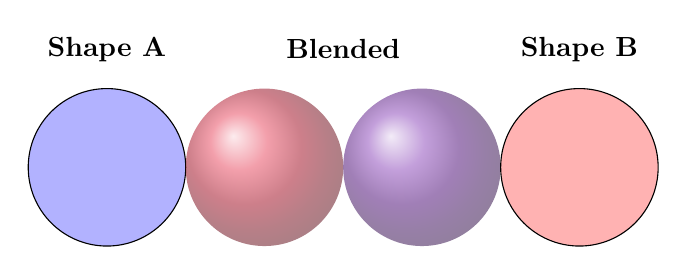
\begin{tikzpicture}
  % Left shape
  \begin{scope}[shift={(-3,0)}]
    \node at (0,1.5) {\textbf{Shape A}};
    \draw[fill=blue!30] (0,0) circle (1);
  \end{scope}

  % Right shape
  \begin{scope}[shift={(3,0)}]
    \node at (0,1.5) {\textbf{Shape B}};
    \draw[fill=red!30] (0,0) circle (1);
  \end{scope}

  % Blended shape
  \begin{scope}[shift={(0,0)}]
    \node at (0,1.5) {\textbf{Blended}};
    \shade[ball color=purple!50!red, opacity=0.5] (-1,0) circle (1);
    \shade[ball color=purple!50!blue, opacity=0.5] (1,0) circle (1);
  \end{scope}
\end{tikzpicture}
